
%(BEGIN_QUESTION)
% Copyright 2014, Tony R. Kuphaldt, released under the Creative Commons Attribution License (v 1.0)
% This means you may do almost anything with this work of mine, so long as you give me proper credit

Sketch phasor diagrams for both phase voltage and phase current in this balanced 3-phase power system:

$$\includegraphics[width=15.5cm]{i00833x01.eps}$$

\vskip 10pt

Now suppose the load is removed from this system and a low-resistance fault appears between phases B and C.  Sketch phasor diagrams for both phase voltage and phase current, assuming the source generator is ``stiff'' (i.e. its voltage does not sag appreciably even under heavy loads):

$$\includegraphics[width=15.5cm]{i00833x03.eps}$$

\underbar{file i00833}
%(END_QUESTION)





%(BEGIN_ANSWER)

Since we know resistors impart no phase shift between voltage and current, the phase angle of each phase voltage remains preserved in the respective phase currents:

$$I_A = {V_A \over R_A} = {120 \hbox{ V} \angle 120^o \over 35 \> \Omega \angle 0^o} = 3.43 \hbox{ A} \angle 120^o$$

$$I_B = {V_B \over R_B} = {120 \hbox{ V} \angle -120^o \over 35 \> \Omega \angle 0^o} = 3.43 \hbox{ A} \angle -120^o$$

$$I_C = {V_C \over R_C} = {120 \hbox{ V} \angle 0^o \over 35 \> \Omega \angle 0^o} = 3.43 \hbox{ A} \angle 0^o$$

$$\includegraphics[width=15.5cm]{i00833x02.eps}$$

\vskip 10pt

\filbreak

The situation with a line-to-line resistive fault is a bit different.  First, the resistance in question sees full line voltage (208 volts) not phase voltage (120 volts).  Next is the fact that the phase angle of this voltage is entirely different: being a phasor stretching between the B and C phasor end-points, $V_{BC}$ (red lead on B, black lead on C) it has a phase angle of $-150^o$.

Calculating phase current through conductor B is as simple as dividing $V_{BC}$ by the fault resistance of 0.25 $\Omega$:

$$I_B = {V_{BC} \over R_{fault}} = {208 \hbox{ V} \angle -150^o \over 0.25 \> \Omega \angle 0^o} = 832 \hbox{ A} \angle -150^o$$

Calculating phase current through conductor C requires we view the fault voltage from that phase's perspective.  $V_{CB}$ is pointed exactly opposite that of $V_{BC}$ and therefore has an angle of +30$^{o}$ rather than $-150^o$.  Applying Ohm's Law again:

$$I_C = {V_{CB} \over R_{fault}} = {208 \hbox{ V} \angle 30^o \over 0.25 \> \Omega \angle 0^o} = 832 \hbox{ A} \angle 30^o$$

$$\includegraphics[width=15.5cm]{i00833x04.eps}$$

There is no phasor shown for conductor A because with no connection to that line $I_A = 0$.

%(END_ANSWER)





%(BEGIN_NOTES)


%INDEX% Electronics review: 3-phase electrical power 
%INDEX% Electronics review, phasor expressions of circuit quantities

%(END_NOTES)


